% Created by tikzDevice version 0.12.3.2 on 2022-02-18 12:00:26
% !TEX encoding = UTF-8 Unicode
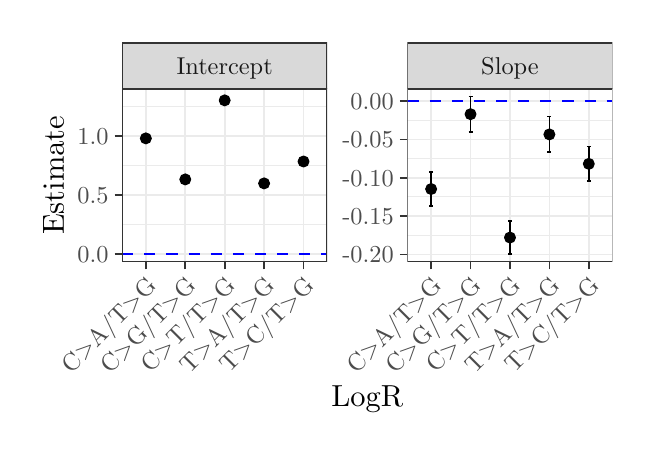
\begin{tikzpicture}[x=1pt,y=1pt]
\definecolor{fillColor}{RGB}{255,255,255}
\path[use as bounding box,fill=fillColor,fill opacity=0.00] (0,0) rectangle (216.81,144.54);
\begin{scope}
\path[clip] (  0.00,  0.00) rectangle (216.81,144.54);
\definecolor{drawColor}{RGB}{255,255,255}
\definecolor{fillColor}{RGB}{255,255,255}

\path[draw=drawColor,line width= 0.6pt,line join=round,line cap=round,fill=fillColor] (  0.00,  0.00) rectangle (216.81,144.54);
\end{scope}
\begin{scope}
\path[clip] ( 34.16, 59.95) rectangle (108.22,122.47);
\definecolor{fillColor}{RGB}{255,255,255}

\path[fill=fillColor] ( 34.16, 59.95) rectangle (108.22,122.47);
\definecolor{drawColor}{gray}{0.92}

\path[draw=drawColor,line width= 0.3pt,line join=round] ( 34.16, 73.44) --
	(108.22, 73.44);

\path[draw=drawColor,line width= 0.3pt,line join=round] ( 34.16, 94.73) --
	(108.22, 94.73);

\path[draw=drawColor,line width= 0.3pt,line join=round] ( 34.16,116.02) --
	(108.22,116.02);

\path[draw=drawColor,line width= 0.6pt,line join=round] ( 34.16, 62.79) --
	(108.22, 62.79);

\path[draw=drawColor,line width= 0.6pt,line join=round] ( 34.16, 84.08) --
	(108.22, 84.08);

\path[draw=drawColor,line width= 0.6pt,line join=round] ( 34.16,105.38) --
	(108.22,105.38);

\path[draw=drawColor,line width= 0.6pt,line join=round] ( 42.70, 59.95) --
	( 42.70,122.47);

\path[draw=drawColor,line width= 0.6pt,line join=round] ( 56.95, 59.95) --
	( 56.95,122.47);

\path[draw=drawColor,line width= 0.6pt,line join=round] ( 71.19, 59.95) --
	( 71.19,122.47);

\path[draw=drawColor,line width= 0.6pt,line join=round] ( 85.43, 59.95) --
	( 85.43,122.47);

\path[draw=drawColor,line width= 0.6pt,line join=round] ( 99.68, 59.95) --
	( 99.68,122.47);
\definecolor{drawColor}{RGB}{0,0,255}

\path[draw=drawColor,line width= 0.6pt,dash pattern=on 4pt off 4pt ,line join=round] ( 34.16, 62.79) -- (108.22, 62.79);
\definecolor{drawColor}{RGB}{0,0,0}
\definecolor{fillColor}{RGB}{0,0,0}

\path[draw=drawColor,line width= 0.4pt,line join=round,line cap=round,fill=fillColor] ( 42.70,104.54) circle (  1.96);

\path[draw=drawColor,line width= 0.4pt,line join=round,line cap=round,fill=fillColor] ( 56.95, 89.71) circle (  1.96);

\path[draw=drawColor,line width= 0.4pt,line join=round,line cap=round,fill=fillColor] ( 71.19,118.27) circle (  1.96);

\path[draw=drawColor,line width= 0.4pt,line join=round,line cap=round,fill=fillColor] ( 85.43, 88.27) circle (  1.96);

\path[draw=drawColor,line width= 0.4pt,line join=round,line cap=round,fill=fillColor] ( 99.68, 96.18) circle (  1.96);

\path[draw=drawColor,line width= 0.6pt,line join=round] ( 41.99,105.65) --
	( 43.41,105.65);

\path[draw=drawColor,line width= 0.6pt,line join=round] ( 42.70,105.65) --
	( 42.70,103.43);

\path[draw=drawColor,line width= 0.6pt,line join=round] ( 41.99,103.43) --
	( 43.41,103.43);

\path[draw=drawColor,line width= 0.6pt,line join=round] ( 56.23, 90.70) --
	( 57.66, 90.70);

\path[draw=drawColor,line width= 0.6pt,line join=round] ( 56.95, 90.70) --
	( 56.95, 88.72);

\path[draw=drawColor,line width= 0.6pt,line join=round] ( 56.23, 88.72) --
	( 57.66, 88.72);

\path[draw=drawColor,line width= 0.6pt,line join=round] ( 70.48,119.63) --
	( 71.90,119.63);

\path[draw=drawColor,line width= 0.6pt,line join=round] ( 71.19,119.63) --
	( 71.19,116.92);

\path[draw=drawColor,line width= 0.6pt,line join=round] ( 70.48,116.92) --
	( 71.90,116.92);

\path[draw=drawColor,line width= 0.6pt,line join=round] ( 84.72, 89.14) --
	( 86.14, 89.14);

\path[draw=drawColor,line width= 0.6pt,line join=round] ( 85.43, 89.14) --
	( 85.43, 87.40);

\path[draw=drawColor,line width= 0.6pt,line join=round] ( 84.72, 87.40) --
	( 86.14, 87.40);

\path[draw=drawColor,line width= 0.6pt,line join=round] ( 98.96, 96.93) --
	(100.39, 96.93);

\path[draw=drawColor,line width= 0.6pt,line join=round] ( 99.68, 96.93) --
	( 99.68, 95.42);

\path[draw=drawColor,line width= 0.6pt,line join=round] ( 98.96, 95.42) --
	(100.39, 95.42);
\definecolor{drawColor}{gray}{0.20}

\path[draw=drawColor,line width= 0.6pt,line join=round,line cap=round] ( 34.16, 59.95) rectangle (108.22,122.47);
\end{scope}
\begin{scope}
\path[clip] (137.24, 59.95) rectangle (211.31,122.47);
\definecolor{fillColor}{RGB}{255,255,255}

\path[fill=fillColor] (137.24, 59.95) rectangle (211.31,122.47);
\definecolor{drawColor}{gray}{0.92}

\path[draw=drawColor,line width= 0.3pt,line join=round] (137.24, 69.55) --
	(211.31, 69.55);

\path[draw=drawColor,line width= 0.3pt,line join=round] (137.24, 83.39) --
	(211.31, 83.39);

\path[draw=drawColor,line width= 0.3pt,line join=round] (137.24, 97.22) --
	(211.31, 97.22);

\path[draw=drawColor,line width= 0.3pt,line join=round] (137.24,111.06) --
	(211.31,111.06);

\path[draw=drawColor,line width= 0.6pt,line join=round] (137.24, 62.63) --
	(211.31, 62.63);

\path[draw=drawColor,line width= 0.6pt,line join=round] (137.24, 76.47) --
	(211.31, 76.47);

\path[draw=drawColor,line width= 0.6pt,line join=round] (137.24, 90.30) --
	(211.31, 90.30);

\path[draw=drawColor,line width= 0.6pt,line join=round] (137.24,104.14) --
	(211.31,104.14);

\path[draw=drawColor,line width= 0.6pt,line join=round] (137.24,117.98) --
	(211.31,117.98);

\path[draw=drawColor,line width= 0.6pt,line join=round] (145.79, 59.95) --
	(145.79,122.47);

\path[draw=drawColor,line width= 0.6pt,line join=round] (160.03, 59.95) --
	(160.03,122.47);

\path[draw=drawColor,line width= 0.6pt,line join=round] (174.28, 59.95) --
	(174.28,122.47);

\path[draw=drawColor,line width= 0.6pt,line join=round] (188.52, 59.95) --
	(188.52,122.47);

\path[draw=drawColor,line width= 0.6pt,line join=round] (202.76, 59.95) --
	(202.76,122.47);
\definecolor{drawColor}{RGB}{0,0,255}

\path[draw=drawColor,line width= 0.6pt,dash pattern=on 4pt off 4pt ,line join=round] (137.24,117.98) -- (211.31,117.98);
\definecolor{drawColor}{RGB}{0,0,0}
\definecolor{fillColor}{RGB}{0,0,0}

\path[draw=drawColor,line width= 0.4pt,line join=round,line cap=round,fill=fillColor] (145.79, 86.23) circle (  1.96);

\path[draw=drawColor,line width= 0.4pt,line join=round,line cap=round,fill=fillColor] (160.03,113.28) circle (  1.96);

\path[draw=drawColor,line width= 0.4pt,line join=round,line cap=round,fill=fillColor] (174.28, 68.70) circle (  1.96);

\path[draw=drawColor,line width= 0.4pt,line join=round,line cap=round,fill=fillColor] (188.52,105.97) circle (  1.96);

\path[draw=drawColor,line width= 0.4pt,line join=round,line cap=round,fill=fillColor] (202.76, 95.33) circle (  1.96);

\path[draw=drawColor,line width= 0.6pt,line join=round] (145.08, 92.33) --
	(146.50, 92.33);

\path[draw=drawColor,line width= 0.6pt,line join=round] (145.79, 92.33) --
	(145.79, 80.13);

\path[draw=drawColor,line width= 0.6pt,line join=round] (145.08, 80.13) --
	(146.50, 80.13);

\path[draw=drawColor,line width= 0.6pt,line join=round] (159.32,119.63) --
	(160.75,119.63);

\path[draw=drawColor,line width= 0.6pt,line join=round] (160.03,119.63) --
	(160.03,106.93);

\path[draw=drawColor,line width= 0.6pt,line join=round] (159.32,106.93) --
	(160.75,106.93);

\path[draw=drawColor,line width= 0.6pt,line join=round] (173.57, 74.61) --
	(174.99, 74.61);

\path[draw=drawColor,line width= 0.6pt,line join=round] (174.28, 74.61) --
	(174.28, 62.79);

\path[draw=drawColor,line width= 0.6pt,line join=round] (173.57, 62.79) --
	(174.99, 62.79);

\path[draw=drawColor,line width= 0.6pt,line join=round] (187.81,112.39) --
	(189.23,112.39);

\path[draw=drawColor,line width= 0.6pt,line join=round] (188.52,112.39) --
	(188.52, 99.56);

\path[draw=drawColor,line width= 0.6pt,line join=round] (187.81, 99.56) --
	(189.23, 99.56);

\path[draw=drawColor,line width= 0.6pt,line join=round] (202.05,101.58) --
	(203.48,101.58);

\path[draw=drawColor,line width= 0.6pt,line join=round] (202.76,101.58) --
	(202.76, 89.08);

\path[draw=drawColor,line width= 0.6pt,line join=round] (202.05, 89.08) --
	(203.48, 89.08);
\definecolor{drawColor}{gray}{0.20}

\path[draw=drawColor,line width= 0.6pt,line join=round,line cap=round] (137.24, 59.95) rectangle (211.31,122.47);
\end{scope}
\begin{scope}
\path[clip] ( 34.16,122.47) rectangle (108.22,139.04);
\definecolor{drawColor}{gray}{0.20}
\definecolor{fillColor}{gray}{0.85}

\path[draw=drawColor,line width= 0.6pt,line join=round,line cap=round,fill=fillColor] ( 34.16,122.47) rectangle (108.22,139.04);
\definecolor{drawColor}{gray}{0.10}

\node[text=drawColor,anchor=base,inner sep=0pt, outer sep=0pt, scale=  0.88] at ( 71.19,127.72) {Intercept};
\end{scope}
\begin{scope}
\path[clip] (137.24,122.47) rectangle (211.31,139.04);
\definecolor{drawColor}{gray}{0.20}
\definecolor{fillColor}{gray}{0.85}

\path[draw=drawColor,line width= 0.6pt,line join=round,line cap=round,fill=fillColor] (137.24,122.47) rectangle (211.31,139.04);
\definecolor{drawColor}{gray}{0.10}

\node[text=drawColor,anchor=base,inner sep=0pt, outer sep=0pt, scale=  0.88] at (174.28,127.72) {Slope};
\end{scope}
\begin{scope}
\path[clip] (  0.00,  0.00) rectangle (216.81,144.54);
\definecolor{drawColor}{gray}{0.20}

\path[draw=drawColor,line width= 0.6pt,line join=round] ( 42.70, 57.20) --
	( 42.70, 59.95);

\path[draw=drawColor,line width= 0.6pt,line join=round] ( 56.95, 57.20) --
	( 56.95, 59.95);

\path[draw=drawColor,line width= 0.6pt,line join=round] ( 71.19, 57.20) --
	( 71.19, 59.95);

\path[draw=drawColor,line width= 0.6pt,line join=round] ( 85.43, 57.20) --
	( 85.43, 59.95);

\path[draw=drawColor,line width= 0.6pt,line join=round] ( 99.68, 57.20) --
	( 99.68, 59.95);
\end{scope}
\begin{scope}
\path[clip] (  0.00,  0.00) rectangle (216.81,144.54);
\definecolor{drawColor}{gray}{0.30}

\node[text=drawColor,rotate= 45.00,anchor=base east,inner sep=0pt, outer sep=0pt, scale=  0.88] at ( 46.99, 50.71) {C$>$A/T$>$G};

\node[text=drawColor,rotate= 45.00,anchor=base east,inner sep=0pt, outer sep=0pt, scale=  0.88] at ( 61.23, 50.71) {C$>$G/T$>$G};

\node[text=drawColor,rotate= 45.00,anchor=base east,inner sep=0pt, outer sep=0pt, scale=  0.88] at ( 75.47, 50.71) {C$>$T/T$>$G};

\node[text=drawColor,rotate= 45.00,anchor=base east,inner sep=0pt, outer sep=0pt, scale=  0.88] at ( 89.72, 50.71) {T$>$A/T$>$G};

\node[text=drawColor,rotate= 45.00,anchor=base east,inner sep=0pt, outer sep=0pt, scale=  0.88] at (103.96, 50.71) {T$>$C/T$>$G};
\end{scope}
\begin{scope}
\path[clip] (  0.00,  0.00) rectangle (216.81,144.54);
\definecolor{drawColor}{gray}{0.20}

\path[draw=drawColor,line width= 0.6pt,line join=round] (145.79, 57.20) --
	(145.79, 59.95);

\path[draw=drawColor,line width= 0.6pt,line join=round] (160.03, 57.20) --
	(160.03, 59.95);

\path[draw=drawColor,line width= 0.6pt,line join=round] (174.28, 57.20) --
	(174.28, 59.95);

\path[draw=drawColor,line width= 0.6pt,line join=round] (188.52, 57.20) --
	(188.52, 59.95);

\path[draw=drawColor,line width= 0.6pt,line join=round] (202.76, 57.20) --
	(202.76, 59.95);
\end{scope}
\begin{scope}
\path[clip] (  0.00,  0.00) rectangle (216.81,144.54);
\definecolor{drawColor}{gray}{0.30}

\node[text=drawColor,rotate= 45.00,anchor=base east,inner sep=0pt, outer sep=0pt, scale=  0.88] at (150.08, 50.71) {C$>$A/T$>$G};

\node[text=drawColor,rotate= 45.00,anchor=base east,inner sep=0pt, outer sep=0pt, scale=  0.88] at (164.32, 50.71) {C$>$G/T$>$G};

\node[text=drawColor,rotate= 45.00,anchor=base east,inner sep=0pt, outer sep=0pt, scale=  0.88] at (178.56, 50.71) {C$>$T/T$>$G};

\node[text=drawColor,rotate= 45.00,anchor=base east,inner sep=0pt, outer sep=0pt, scale=  0.88] at (192.81, 50.71) {T$>$A/T$>$G};

\node[text=drawColor,rotate= 45.00,anchor=base east,inner sep=0pt, outer sep=0pt, scale=  0.88] at (207.05, 50.71) {T$>$C/T$>$G};
\end{scope}
\begin{scope}
\path[clip] (  0.00,  0.00) rectangle (216.81,144.54);
\definecolor{drawColor}{gray}{0.30}

\node[text=drawColor,anchor=base east,inner sep=0pt, outer sep=0pt, scale=  0.88] at (132.29, 59.60) {-0.20};

\node[text=drawColor,anchor=base east,inner sep=0pt, outer sep=0pt, scale=  0.88] at (132.29, 73.44) {-0.15};

\node[text=drawColor,anchor=base east,inner sep=0pt, outer sep=0pt, scale=  0.88] at (132.29, 87.27) {-0.10};

\node[text=drawColor,anchor=base east,inner sep=0pt, outer sep=0pt, scale=  0.88] at (132.29,101.11) {-0.05};

\node[text=drawColor,anchor=base east,inner sep=0pt, outer sep=0pt, scale=  0.88] at (132.29,114.95) {0.00};
\end{scope}
\begin{scope}
\path[clip] (  0.00,  0.00) rectangle (216.81,144.54);
\definecolor{drawColor}{gray}{0.20}

\path[draw=drawColor,line width= 0.6pt,line join=round] (134.49, 62.63) --
	(137.24, 62.63);

\path[draw=drawColor,line width= 0.6pt,line join=round] (134.49, 76.47) --
	(137.24, 76.47);

\path[draw=drawColor,line width= 0.6pt,line join=round] (134.49, 90.30) --
	(137.24, 90.30);

\path[draw=drawColor,line width= 0.6pt,line join=round] (134.49,104.14) --
	(137.24,104.14);

\path[draw=drawColor,line width= 0.6pt,line join=round] (134.49,117.98) --
	(137.24,117.98);
\end{scope}
\begin{scope}
\path[clip] (  0.00,  0.00) rectangle (216.81,144.54);
\definecolor{drawColor}{gray}{0.30}

\node[text=drawColor,anchor=base east,inner sep=0pt, outer sep=0pt, scale=  0.88] at ( 29.21, 59.76) {0.0};

\node[text=drawColor,anchor=base east,inner sep=0pt, outer sep=0pt, scale=  0.88] at ( 29.21, 81.05) {0.5};

\node[text=drawColor,anchor=base east,inner sep=0pt, outer sep=0pt, scale=  0.88] at ( 29.21,102.35) {1.0};
\end{scope}
\begin{scope}
\path[clip] (  0.00,  0.00) rectangle (216.81,144.54);
\definecolor{drawColor}{gray}{0.20}

\path[draw=drawColor,line width= 0.6pt,line join=round] ( 31.41, 62.79) --
	( 34.16, 62.79);

\path[draw=drawColor,line width= 0.6pt,line join=round] ( 31.41, 84.08) --
	( 34.16, 84.08);

\path[draw=drawColor,line width= 0.6pt,line join=round] ( 31.41,105.38) --
	( 34.16,105.38);
\end{scope}
\begin{scope}
\path[clip] (  0.00,  0.00) rectangle (216.81,144.54);
\definecolor{drawColor}{RGB}{0,0,0}

\node[text=drawColor,anchor=base,inner sep=0pt, outer sep=0pt, scale=  1.10] at (122.73,  7.64) {LogR};
\end{scope}
\begin{scope}
\path[clip] (  0.00,  0.00) rectangle (216.81,144.54);
\definecolor{drawColor}{RGB}{0,0,0}

\node[text=drawColor,rotate= 90.00,anchor=base,inner sep=0pt, outer sep=0pt, scale=  1.10] at ( 13.08, 91.21) {Estimate};
\end{scope}
\end{tikzpicture}
